\documentclass[11pt,a4paper]{article}
\usepackage[margin=2.2cm]{geometry}
\usepackage[T1]{fontenc}
\usepackage{charter}
\usepackage{microtype}
\usepackage{graphicx}
\usepackage{booktabs}
\usepackage{array}
\usepackage{tabularx}
\usepackage{float}
\usepackage{caption}
\usepackage{enumitem}
\usepackage{amsmath}
\usepackage[table]{xcolor}
\usepackage{listings}
\usepackage[most]{tcolorbox}
\usepackage{fancyhdr}
\usepackage[colorlinks=true,linkcolor=accent,urlcolor=accent]{hyperref}

\definecolor{accent}{HTML}{3C3489}
\definecolor{codebg}{HTML}{F6F6F3}
\definecolor{kw}{HTML}{185FA5}
\definecolor{cm}{HTML}{6B6A64}
\definecolor{okgreen}{HTML}{0F6E56}
\definecolor{badred}{HTML}{A32D2D}

\setlength{\parindent}{0pt}
\setlength{\parskip}{6pt}
\setlist{itemsep=2pt,topsep=4pt}
\captionsetup{font=small,labelfont=bf}
\renewcommand{\arraystretch}{1.18}

\pagestyle{fancy}\fancyhf{}
\rhead{\small\color{cm}\reporttag}
\cfoot{\small\thepage}
\renewcommand{\headrulewidth}{0.3pt}

\lstdefinelanguage{SV}{
  morekeywords={module,endmodule,input,output,inout,logic,wire,reg,always_ff,always_comb,assign,
    begin,end,if,else,case,endcase,default,typedef,enum,localparam,posedge,negedge,or,task,endtask,
    function,endfunction,automatic,initial,repeat,while,for,integer,string,signed,void},
  sensitive=true, morecomment=[l]{//}, morecomment=[s]{/*}{*/}, morestring=[b]"}
\lstdefinelanguage{ICCTcl}{
  morekeywords={set_app_var,create_mw_lib,open_mw_lib,import_designs,read_sdc,set_tlu_plus_files,
    save_mw_cel,create_floorplan,derive_pg_connection,create_rectangular_ring,create_power_strap,
    create_fp_placement,place_opt,clock_opt,report_placement_utilization,report_qor,report_timing,
    insert_stdcell_filler,route_opt,verify_zrt_route,extract_rc,write_parasitics,write_verilog,
    close_mw_cel,gui_start,set_dont_use,get_lib_cells},
  sensitive=true, morecomment=[l]{\#}}
\lstset{basicstyle=\ttfamily\footnotesize, backgroundcolor=\color{codebg}, frame=single,
  rulecolor=\color{codebg}, keywordstyle=\color{kw}\bfseries, commentstyle=\color{cm}\itshape,
  columns=fullflexible, keepspaces=true, breaklines=true, showstringspaces=false,
  xleftmargin=4pt, xrightmargin=4pt, aboveskip=6pt, belowskip=6pt}

\newtcolorbox{task}{colback=accent!5,colframe=accent,boxrule=0.6pt,arc=2pt,
  left=8pt,right=8pt,top=4pt,bottom=4pt,fonttitle=\bfseries,title=The assignment}
\newtcolorbox{keypoint}[1]{colback=okgreen!6,colframe=okgreen,boxrule=0.6pt,arc=2pt,
  left=8pt,right=8pt,top=4pt,bottom=4pt,fonttitle=\bfseries,title={#1}}
\newtcolorbox{lesson}[1]{colback=orange!7,colframe=orange!70!black,boxrule=0.6pt,arc=2pt,
  left=8pt,right=8pt,top=4pt,bottom=4pt,fonttitle=\bfseries,title={#1}}

\newcommand{\fig}[3]{\begin{figure}[H]\centering\includegraphics[width=#2\linewidth]{figures/#1}\caption{#3}\end{figure}}
\newcommand{\met}{\textcolor{okgreen}{\textbf{MET}}}
\newcommand{\viol}{\textcolor{badred}{\textbf{VIOLATED}}}
% numbers still to be copied from my own .rpt files (shows in red until filled in)
\newcommand{\fillin}[1]{\textcolor{badred}{\textbf{[#1]}}}

\newcommand{\header}[3]{%
  \begin{center}
  {\small\color{cm} CPE 527 VLSI Design \quad|\quad Lab 3 \quad|\quad University of Alabama in Huntsville}\\[8pt]
  {\LARGE\bfseries\color{accent} #1}\\[4pt]
  {\large #2}\\[8pt]
  {\small Bibek Shrestha \quad|\quad October 2026 \quad|\quad #3}
  \end{center}\vspace{2pt}\hrule\vspace{6pt}}
\newcommand{\reporttag}{Lab 3 / Assignment 2: serial adder place and route}
\begin{document}
\header{Place and Route of the 8-bit Bit-Serial Adder}{Taking the Lab 2 netlist through IC Compiler}{Synopsys IC Compiler, SAED 90\,nm}

\begin{task}
Run the IC Compiler flow from the tutorial on a design from the previous lab: floorplan, power plan,
placement, clock tree synthesis and routing. Generate and analyze the reports after CTS and after routing.
\end{task}

\section*{At a glance}
\begin{table}[H]\centering\small
\begin{tabular}{lccc}
\toprule
 & \textbf{Lab 2 (DC)} & \textbf{After CTS} & \textbf{After routing} \\
\midrule
Library corner & typ & max & max \\
Wires & none & estimated & routed + extracted \\
Clock & 5 ns & 5 ns & 5 ns \\
Setup slack & +1.77 ns & \fillin{ns} & \fillin{ns} \\
Violating paths & 0 & \fillin{} & \fillin{} \\
Hold violations & & \fillin{} & \fillin{} \\
Flip-flops & 23 & \fillin{} & \fillin{} \\
Cell area & 1268.12 & \fillin{} & \fillin{} \\
Utilization & & \fillin{\%} & \fillin{\%} \\
Open nets / DRCs & & & \fillin{} / \fillin{} \\
\bottomrule
\end{tabular}
\caption{Lab 2 synthesis next to the two ICC checkpoints.}
\end{table}

\section{The design}
The bit-serial adder from Lab 2 adds two 8-bit numbers with one full adder, one bit per clock.
A 3-state FSM (\texttt{u\_ctrl}) drives a datapath (\texttt{u\_dp}) with two shift registers, a carry
flip-flop and a 4-bit bit counter.

\fig{a2_block.png}{0.78}{Block diagram from Lab 2.}

Ports: \texttt{clk}, \texttt{rst\_n}, \texttt{data\_in[7:0]}, \texttt{data\_out[7:0]}, \texttt{ldA}, \texttt{ldB},
\texttt{clrCarry}, \texttt{setCarry}, \texttt{CarryOut}, \texttt{RDY}: 24 signal pins.

\section{Script}
Same flow as the tutorial. Only the names change: library \texttt{ADDER\_LIB}, design \texttt{adder\_baseline.ddc}
with top \texttt{serial\_adder}, constraints \texttt{adder\_baseline.sdc} (5\,ns), and checkpoints
\texttt{ADDER\_init}, \texttt{ADDER\_cts\_opt}, \texttt{ADDER\_route}. This design has no tri-state bus, so the
BSLEX ban used for the multiplier is not needed here.

\section{Routed layout}
\begin{figure}[H]\centering
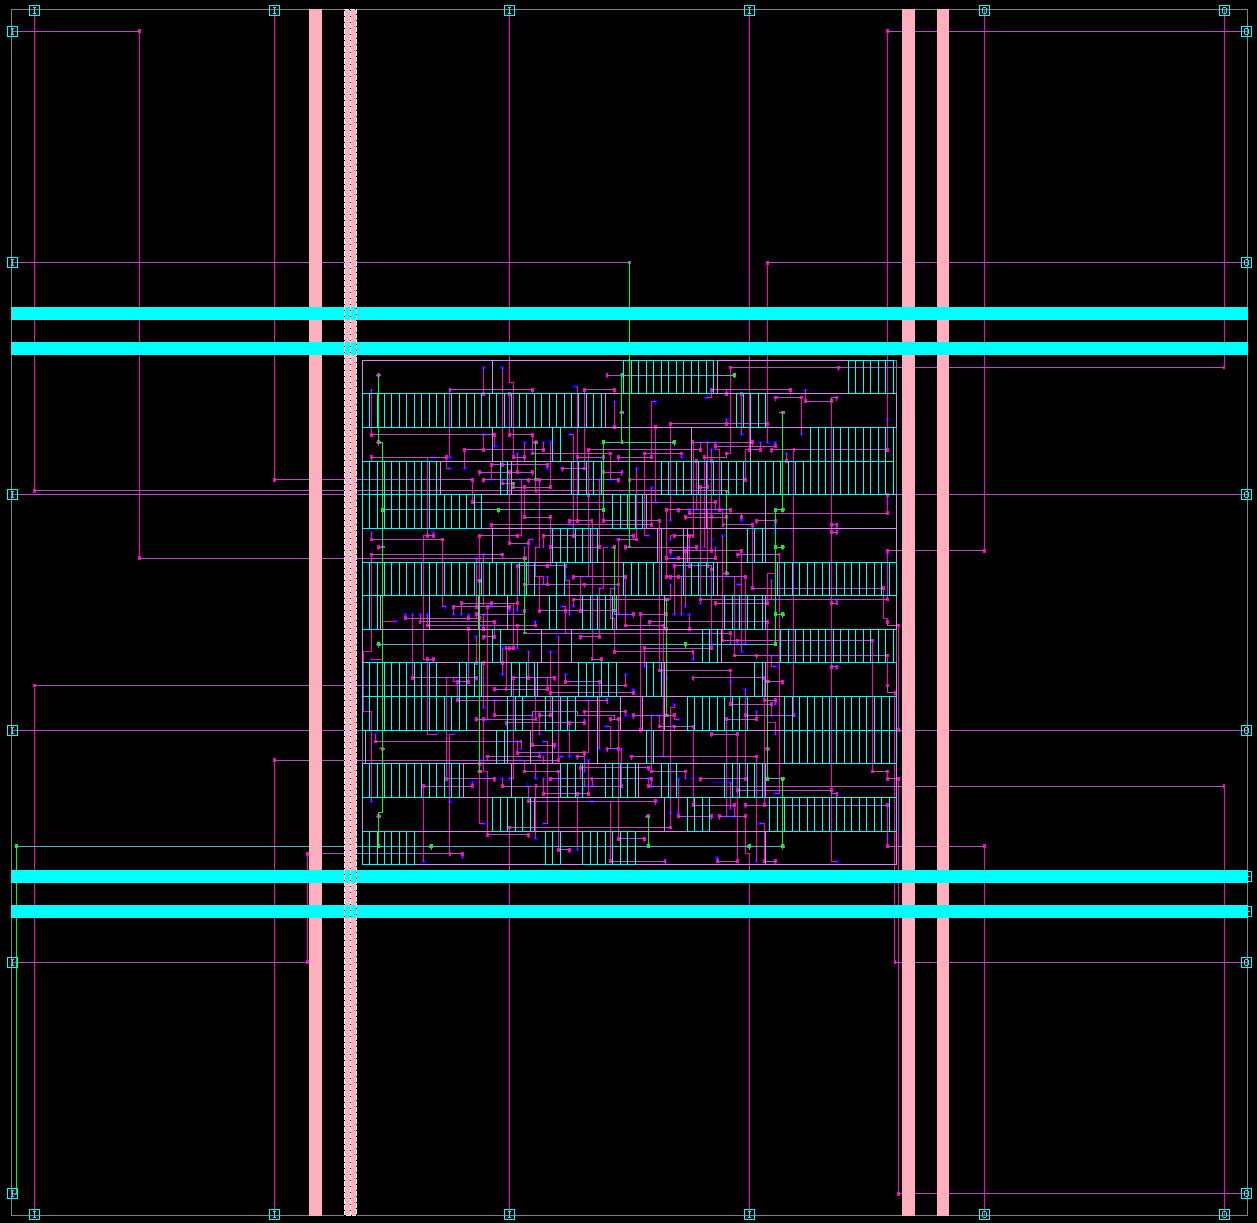
\includegraphics[width=0.49\linewidth]{figures/icc_routed.png}\hfill
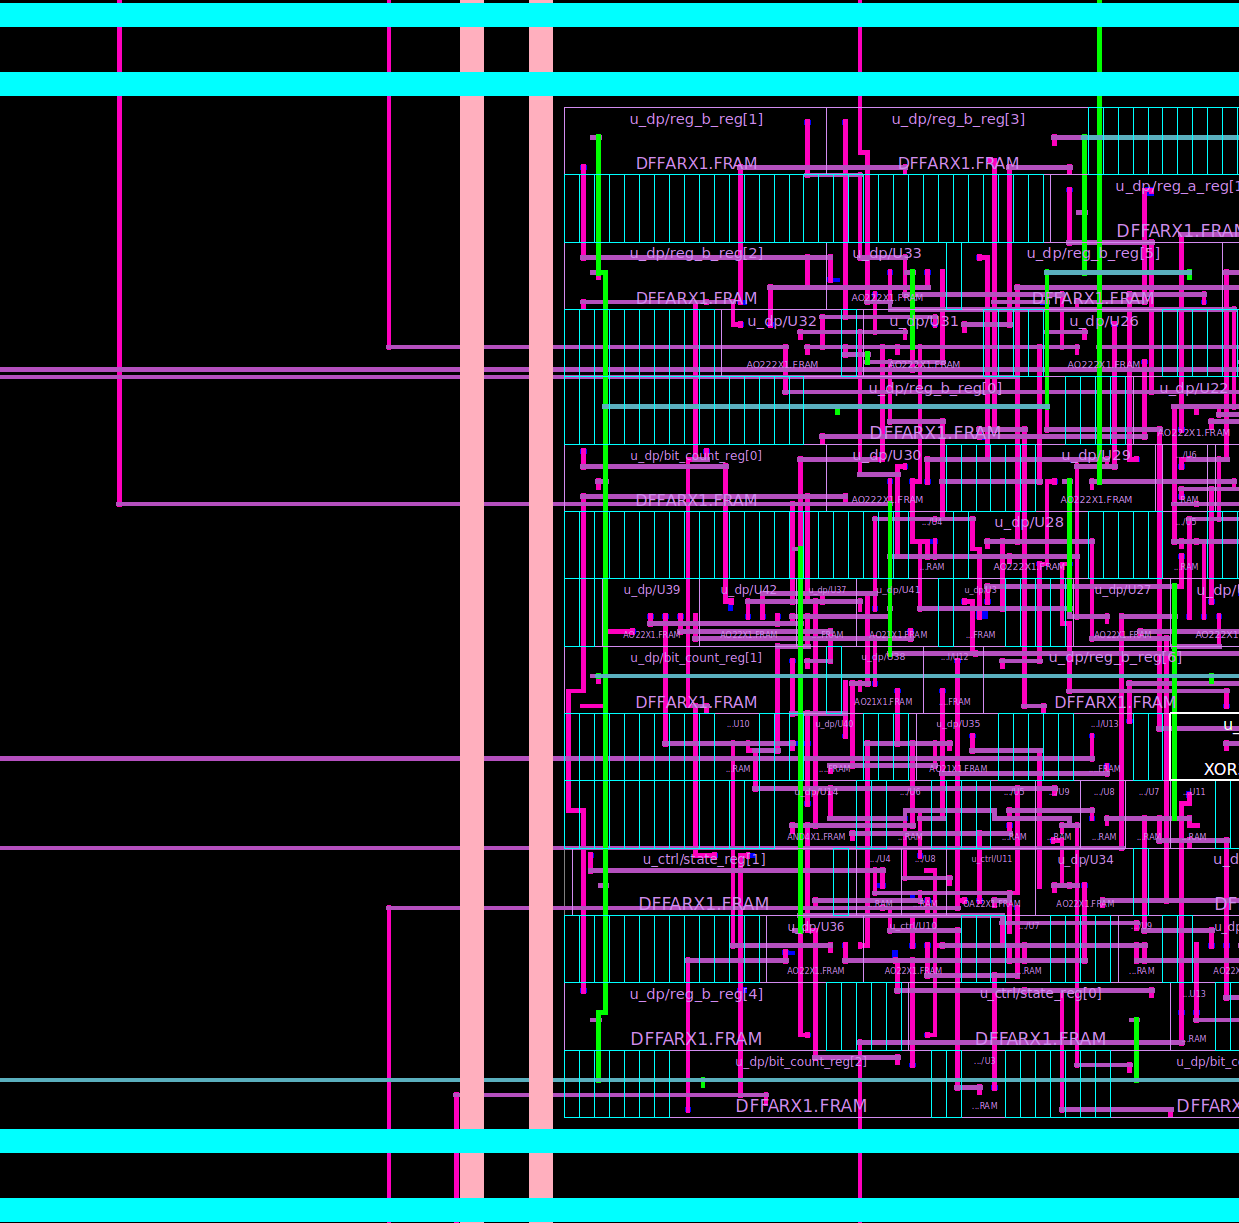
\includegraphics[width=0.49\linewidth]{figures/icc_routed_zoom.png}
\caption{Left: the whole block. Right: the core, with fillers (cyan) between cells.}
\end{figure}

\begin{itemize}
\item \textbf{Ring size.} Querying the left VSS ring segment gives layer M6, width 1.0\,\textmu m and length 103.2\,\textmu m,
      so the ring is about 103\,\textmu m on a side.
\item \textbf{Long I/O wires.} Most of the die is the 30\,\textmu m margin. The 24 signal wires cross it from
      the pins on the die edge to the cells in the core, so for a design this small the I/O wiring is a large share of the total wire length.
\item \textbf{All 23 flip-flops are visible}, the same count as in Lab 2:
\begin{center}\small
\begin{tabular}{lc}
\texttt{u\_dp/reg\_a\_reg[0..7]} & 8 \\
\texttt{u\_dp/reg\_b\_reg[0..7]} & 8 \\
\texttt{u\_dp/bit\_count\_reg[0..3]} & 4 \\
\texttt{u\_dp/carry\_reg\_reg} & 1 \\
\texttt{u\_ctrl/state\_reg[0..1]} & 2 \\
\end{tabular}
\end{center}
\end{itemize}

\fig{icc_routed_zoom2.png}{0.95}{Closer view. \texttt{u\_dp/U16} is an \texttt{XOR3X1}: the sum bit of the single full adder, $a \oplus b \oplus c$.}

\section{Reports}
\begin{table}[H]\centering\small
\begin{tabular}{lll}
\toprule
Report & What I checked & Result \\
\midrule
\texttt{ADDER\_route\_qor.rpt} & slack, violating paths & \fillin{} \\
\texttt{ADDER\_route.setup.rpt} & worst setup path & \fillin{start $\rightarrow$ end, slack} \\
\texttt{ADDER\_route.hold.rpt} & worst hold path & \fillin{} \\
\texttt{ADDER\_route\_util.rpt} & standard cell utilization & \fillin{} \\
\texttt{verify\_zrt\_route} & open nets, DRCs & \fillin{} \\
\bottomrule
\end{tabular}
\caption{Post-route reports.}
\end{table}

\begin{lesson}{Compared with Lab 2}
In Lab 2 the critical path was control logic (\texttt{ldB} $\rightarrow$ FSM $\rightarrow$ \texttt{bit\_count\_reg[3]}),
not the adder, with +1.77\,ns of slack at the typical corner. After routing at the slow corner the slack is
\fillin{ns}, so the design \fillin{still meets / misses} 5\,ns.
\end{lesson}

\section{Inside the cells}
\begin{figure}[H]\centering
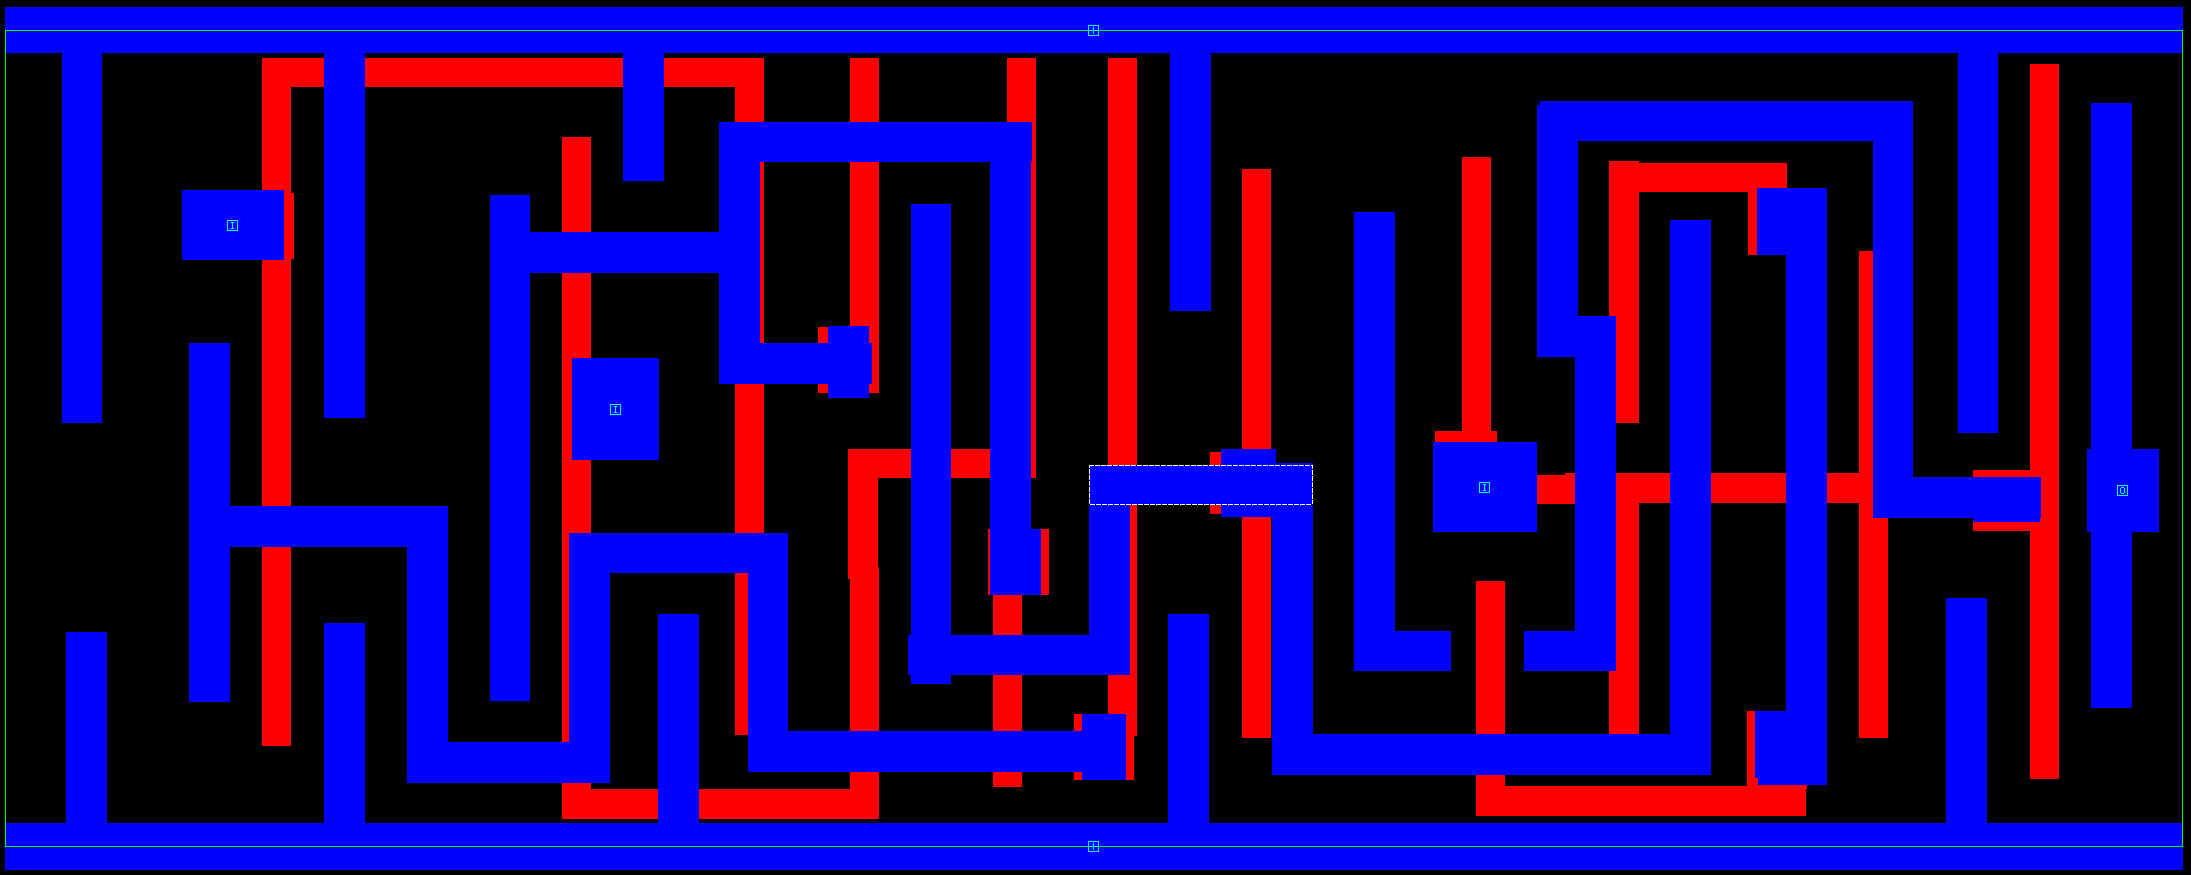
\includegraphics[height=3.6cm]{figures/icc_xor3x1_fram.png}\\[4pt]
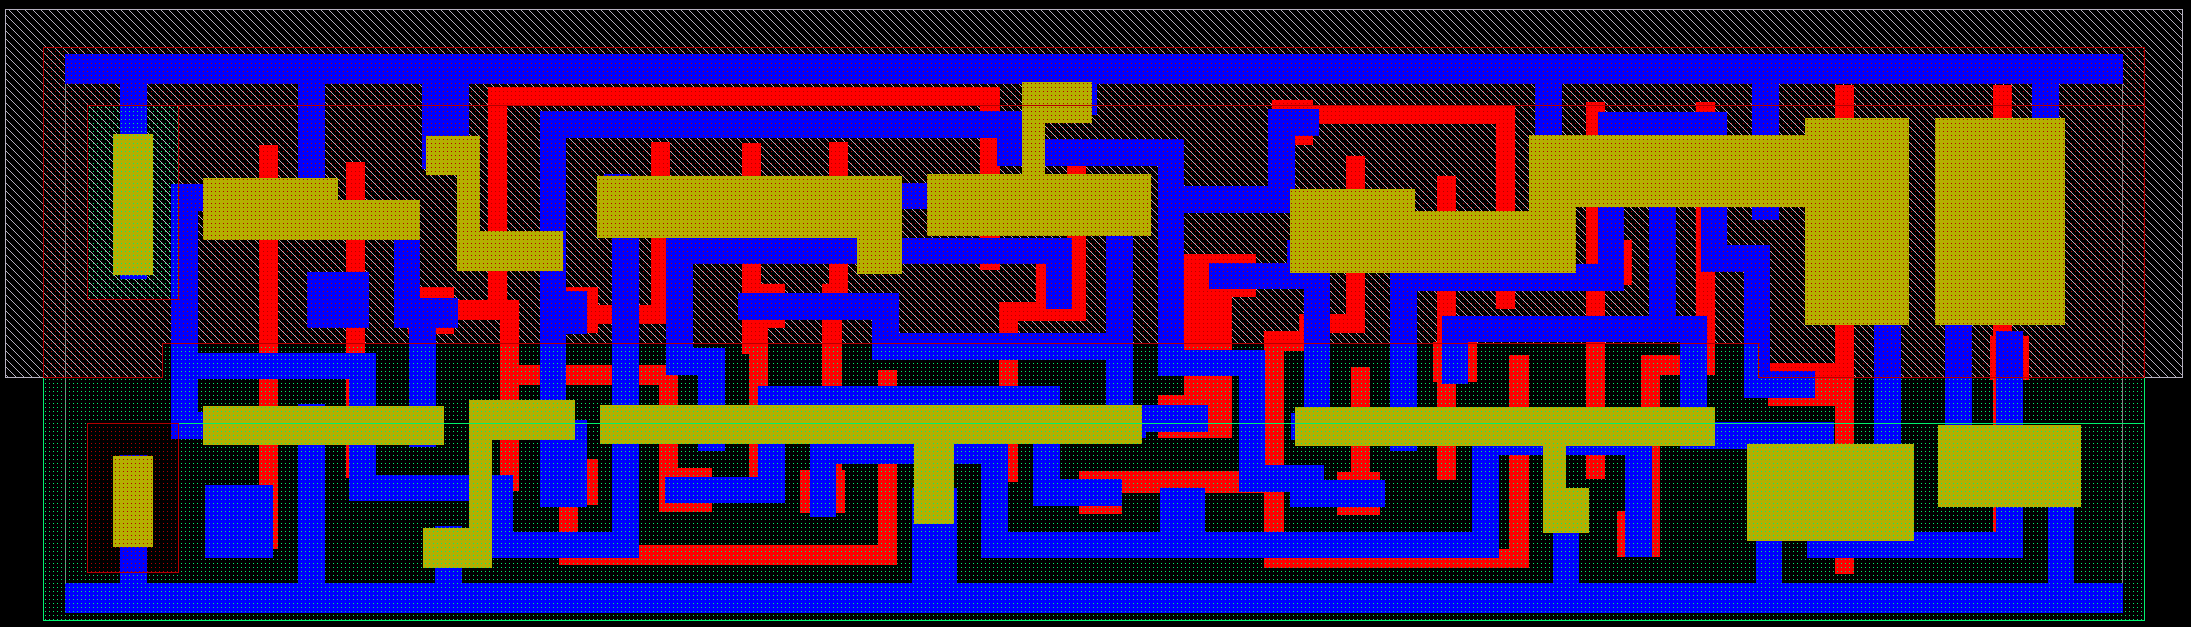
\includegraphics[height=3.6cm]{figures/icc_dffarx1_cel.png}
\caption{Top: \texttt{XOR3X1} FRAM view (the adder's sum cell): rails, metal blockages and four pin squares
(3 inputs, 1 output). Bottom: \texttt{DFFARX1} CEL view, the flip-flop used for all 23 registers. It is much wider
than a logic gate, which is why the flip-flops are the biggest cells in the layout.}
\end{figure}

\section{What I learned}
\begin{itemize}
\item In a small design the core is tiny; the fixed 30\,\textmu m margin and the I/O wires take up most of the die.
\item Every register from the RTL can be found by name in the layout, which makes checking the netlist easy.
\item Flip-flops dominate the area here: 23 of them, each several times wider than an XOR.
\end{itemize}

\appendix
\section{Source files}
\subsection*{RTL: \texttt{src/assignment2.sv}}
\lstinputlisting[language=SV]{src/assignment2.sv}
\subsection*{Testbench: \texttt{src/assignment2\_tb.sv}}
\lstinputlisting[language=SV]{src/assignment2_tb.sv}
\subsection*{ICC script: \texttt{src/icc\_adder.tcl}}
\lstinputlisting[language=ICCTcl]{src/icc_adder.tcl}
\end{document}
